\chapter{A Formal Framework for the Reinforcement Learning of Decision Tree Policies}
\section{Learning Decision Tree policies}
Deicision tree policies offer transparency over neural network policies (cite). 
One can attribute an importance measure to each feature of the state for the deicison of a tree policy which is harder to do for neural networks (cite).

Recently, algorithms have been developed to return decision tree policies for an MDP.
Those algorithms, like any interpretable machine learning method, are either direct or indrect (cite).
We propose an additional distinction amongst the direct methods: algorithms learning parametric trees and algorithms learning non-parametric trees.

Parametric trees are not ``grown'' from the root by iteratively adding internal or leaf nodes depending on the interpretability-performance trade-off to optimize, but are rather ``optimized'': the depth, internal nodes arrengement, and state-features to consider in each nodes are fixed \textit{a priori} and only the tested thresholds of each nodes are optimized similarly to how the weights of a neural network are optimized.
As the reader might have guessed, those parametric trees are advantageous in that they can be learned with gradient descent and in the context of decision tree policies, with the policy gradient (cite).
The downside of those approaches is that a user cannot know \textit{a priori}  what a ``good'' tree policy structure should be for a particular MDP: either the specified structure is too deep and pruning will be required after training or the tree structure is not expressive enough to encode a good policy. 
Similar approaches exist in supervised learning exist where a parametric tree is fitted with gradient descent (cite). However their benefit over non-parametric trees have not been shown.
When parametric trees are learned for MDPs; extra stabilizing tricks are required during training such as adaptive batch sizes (cite).

Non-parametric trees are the standard model in supervised learning (cite) and can naturally trade-off between interpretability and performances. However, specialized approaches are required since growing a tree from the root in an RL fashion is not possible.
In the next section we present, to the best of our knowledge, the only direct approach to learn non-parametric decision tree policies for MDPs; Iterative Bounding Markove Decision Processes (cite). 

Other more specialized approaches deal with tree policies either for specific MDPs like maze (cite) or for very small depth (cite) or when the MDP model is known (cite).

\section{Example of the limitations of indirect methods}
We believe this toy problem can reveal interesting properties of interpretable machine learning methods as this particular base MDP can in fact be optiamlly controlled by a detph-1 decision tree.

\begin{figure}[h]
    \centering
    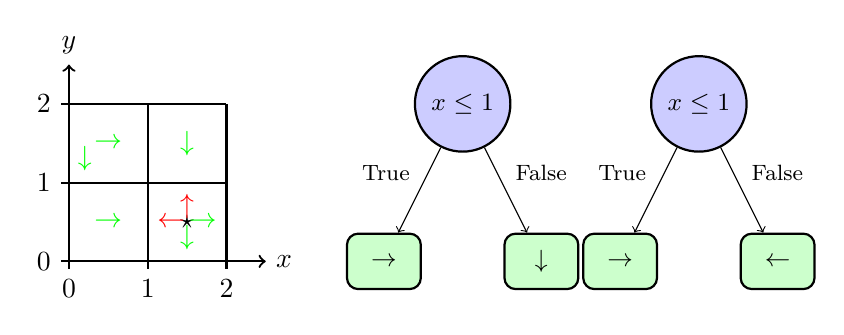
\begin{tikzpicture}[
        decision/.style={circle, draw, thick, fill=blue!20, text width=2.5em, text centered, minimum height=2.5em, font=\small},
        leaf/.style={rectangle, draw, thick, fill=green!20, text width=2em, text centered, rounded corners, minimum height=2em, font=\small},
        edge_label/.style={font=\footnotesize, midway}
    ]
        % Tree 4: if x <= 0.5 move right else move left
        \node[decision] (tree4_root) at (8,2) {$x \leq 1$};
        \node[leaf] (tree4_right) at (7,0) {$\rightarrow$};
        \node[leaf] (tree4_left) at (9,0) {$\leftarrow$};
        \draw[->] (tree4_root) -- (tree4_right) node[edge_label, above left] {True};
        \draw[->] (tree4_root) -- (tree4_left) node[edge_label, above right] {False};
        \tikzstyle{grid}=[draw, thick, fill=gray!10]


        % Tree 4: if x <= 0.5 move right else move left
        \node[decision] (tree5_root) at (5,2) {$x \leq 1$};
        \node[leaf] (tree5_right) at (4,0) {$\rightarrow$};
        \node[leaf] (tree5_left) at (6,0) {$\downarrow$};
        \draw[->] (tree5_root) -- (tree5_right) node[edge_label, above left] {True};
        \draw[->] (tree5_root) -- (tree5_left) node[edge_label, above right] {False};
        \tikzstyle{grid}=[draw, thick, fill=gray!10]
        
        % Draw grid
        \draw[grid] (0,0) grid (2,2);
        
        % Add axes
        \draw[thick, ->] (0,0) -- (2.5,0) node[right] {$x$};
        \draw[thick, ->] (0,0) -- (0,2.5) node[above] {$y$};
        
        % Add tick marks and labels
        \foreach \x in {0,1,2} {
            \draw[thick] (\x,0) -- (\x,-0.1) node[below] {$\x$};
        }
        \foreach \y in {0,1,2} {
            \draw[thick] (0,\y) -- (-0.1,\y) node[left] {$\y$};
        }
        
        % Add state labels clockwise from bottom left
        \node at (0.5,0.5) {{\color{green} $\rightarrow$}};
        \node at (1.5,0.5) {$\star$};
        \node at (1.5,0.7) {{\color{red} $\uparrow$}};
        \node at (1.5,0.3) {{\color{green} $\downarrow$}};
        \node at (1.7,0.5) {{\color{green} $\rightarrow$}};
        \node at (1.3,0.5) {{\color{red} $\leftarrow$}};
        \node at (1.5,1.5) {{\color{green} $\downarrow$}};
        \node at (0.2,1.3) {{\color{green} $\downarrow$}};
        \node at (0.5,1.5) {{\color{green} $\rightarrow$}};

    \end{tikzpicture}
    \caption{Grid world MDP optimal actions. An optimal policy that takes any of the red actions in the bottom right state might not be imitated by the best depth-1 tree in terms of performance interpretability trade-offs.
    Center, an optimal depth-1 decision tree policy. On the right, a sub-optimal depth-1 decision tree policy.}
    \end{figure}

\begin{figure}
    \centering
    \includegraphics[width=0.6\textwidth]{images/images_part1/policy_values_comparison.pdf}
    \caption{MDP objective values.}\label{fig:objectives}
\end{figure}

\begin{figure}
    \centering
    \includegraphics[width=1\textwidth]{images/images_part1/base_mdp.pdf}
    \caption{Left, sample complexity curve of Q-learning with default hyperparameters on the $2\times 2$ grid world MDP over 100 random seeds. Right, performances of indirect interpretable methods when imitating the greedy policy with a tree at different Q-learning stages. }
\end{figure}

\section{Iterative Bounding Markov Decision Processes}
In 2021, Topin et. al. introduced Iterative Bouding Markov Decision Processes (IBMDPs) with the promise of shifting the challenges of non-parametric decision tree policy learning in the problem formulation rather than in the design of specialized reinforcement learning algorithms.
Given a base MDP for which one wants to learn a decision tree policy, IBMDPs are an augmented version of this base MDP with more state features, more actions, additinal reward signal, and additional transition kernel.
Authors showed that certain IBMDP policies, that can be learned with RL, are equivalent to decision tree policies for the base MDP. 
\subsection{Formalism}
The key thing to know about IBMDPs is that they are, as their name suggests, MDPs. Hence they inherit all their properties such as existence of a deterministic optimal Markovian policy.
The states in an IBMDP are concatenations of base MDP states and some observations. Those observations are information about the base states that are refined--``iteratively bounded''-- at each step and represent a subspace of the base MDP state space.
Actions available in an IBMDP are the actions of the base MDP, that change the state of the latter, and \textit{information gathering} actions that change the observation part of the IBMDP state.
Now, taking base actions in an IBMDP is rewarded like in the base MDP, this ensures that the base objective, e.g. balancing the pole or treating cancer, is still encoded in the IBMDP reward. When taking such \textit{information gathering} actions; the reward is an arbitrary value supposed to trade-off between performance and interpretability.
 
Before showing how to get decision trees from IBMDP policies, we give a formal definition of the latter following Topin et. al. (cite).

\begin{definition}[Iterative Bounding Markov decision process]
Given a \textit{factored} (cite) MDP $\mathcal{M}$ (cite), that is, a tuple $\langle S, A, R, T, T_0 \rangle$ with $S\subsetneq \mathbb{R}^n$, an Iterative Bouding MDP $\mathcal{M}_ib$ is a tuple:
\begin{align*}
    \langle \overbrace{S, O}^{\text{State space}}, \underbrace{A, A_{info}}_{\text{Action space}}, \overbrace{R, \zeta}^{\text{Reward function}}, \underbrace{T_{info}, T, T_0}_{\text{Transition kernels}}\rangle
\end{align*}

\begin{itemize}
\item $S$ the base MDP state space should be of the form $S = [L_1, U_1]\times \dots \times [L_n, U_n]$ with $\infty < L_i \leq U_i < \infty \forall 1\leq i\leq n$.
\item $O$ are the observations in an IBMDP. They are partial information about the values of base MDP states: $O\subsetneq S^2 =  [L_1, U_1]\times \dots \times [L_n, U_n] \times [L_1, U_1]\times \dots \times [L_n, U_n]$. So the complete IBMDP state space is $(S, O) = S \times O$ the concatenations of states and observations.
\item $A$ are the actions of the base MDP.
\item $A_{info}$ are added \textit{information gathering} actions (IGAs) of the form $\langle i, v \rangle$ where $i$ is a state feature index $1 \leq i \leq n$ and $v$ is a real number. So the complete action space of an IBMDP is the set of base actions and \textit{information gathering} actions $A \cup A_{info}$.
\item $R: S\times A \rightarrow \mathbb{R}$ is the base MDP reward function that maps base states and actions to a real-valued reward signal.
\item $\zeta$ is a reward signal for taking an \textit{information gathering} action. So the IBMDP reward function is to get a reward from the base MDP if the action is a base MDP action or to get $\zeta$ if the action is a \textit{information gathering} action.
\item $T_{info}: S\times O \times( A_{info} \cup A )\rightarrow \Delta (S\times O)$ is the transition kernel of IBMDPs. 
Given the current observation $o_{t} = (L'_1, U'_1, \dots, L'_n, U'_n)\in O$ and the current state is $s_t=(s_1, s_2, \dots, s_n)$ if an AIG $\langle i, v \rangle$ is taken, only the bounds in the observation change:
\begin{align*}
    o_{t+1} &= \begin{cases}
        (L'_1, U'_1, \dots , L'_i, \min\{v, U'_i\}, \dots , L'_n, U'_n) \text{ if } s_i \leq v\\
        (L'_1, U'_1, \dots , \max\{v, L'_i\}, U'_i, \dots , L'_n, U'_n) \text{ if } s_i > v
    \end{cases}
\end{align*}
If a base action $a\in A$ is taken, $o_{t+1}$ is reset to the default state bounds $(L_1, U_1,\dots, L_n, U_n)$ and the base state changes according to the base MDP transitition kernel: $s_{t+1}\sim T(s, a)$.
At initialization, the base part of the IBMDP states is drawn from $T_0$ and the observation is set always set to $(L_1, U_1,\dots, L_n, U_n)$.
The overall IBMDP transitions are given by either $T_{info}$, which i fully deterministic, if an IGA is played, and by the base MDP's transition kernel otherwise.
\end{itemize}
\end{definition}
Now remains to extract a decision tree policy for $\mathcal{M}$ from a policy for IBMDP $\mathcal{M}_{IB}$. 

\subsection{From Policies to Trees}
\begin{algorithm}[t]
    \KwData{IBMDP policy $\pi$ and observation $o=(L'_1, U'_1, \dots, L'_n, U'_n)$}
    \KwResult{Decision tree policy extracted from $\pi$}
    
    \SetKwProg{Fn}{Function}{:}{}
    \SetKwFunction{SubtreeFromPolicy}{Subtree\_From\_Policy}
    
    \Fn{\SubtreeFromPolicy{$o, \pi$}}{
        $a \leftarrow \pi(o)$ \\
        \If{$a \in A_{info}$}{
            \Return Leaf\_Node(action: $a$) \Comment{// Leaf if base action}
        }
        \Else{
            $\langle i, v\rangle \leftarrow a$ \Comment{// Splitting action is feature and value} \\
            $o_L \leftarrow o; \quad o_R \leftarrow o$ \\
                         $o_L \leftarrow (L'_1, U'_1, \dots, L'_i, v, \dots, L'_n, U'_n); \quad o_R \leftarrow (L'_1, U'_1, \dots, v, U'_i, \dots, L'_n, U'_n)$ \\
            $child_L \leftarrow$ Subtree\_From\_Policy$(o_L, \pi)$ \\
            $child_R \leftarrow$ Subtree\_From\_Policy$(o_R, \pi)$ \\
            \Return Internal\_Node(feature: $i$, value: $v$, children: $(child_L, child_R)$)
        }
    }
    
    \caption{Extract a Decision Tree Policy from an IBMDP policy $\pi$, beginning traversal from $obs$.}\label{alg_extract_tree}
\end{algorithm}

One can notice that \textit{information gathering} actions resemble the Boolean functions that make up internal decision tree nodes (cite). 
Indeed, an agent evolving in an IBMDP essentially builds a tree by taking sequences of IGAs (internal nodes) and then a base action (leaf node) and repeats this process over time.
However not all IBMDP policies are decision tree policies. In particular, only deterministic policies depending solely on the observation part of the IBMDP states $\pi: O \rightarrow A\cup A_{info}$ are decision tree policies $\pi_{\mathcal{T}}: S \rightarrow A$ for the base MDP (cite).
Algorithm (cite) from (cite) extracts a decision tree policy for the base MDP from a determenistic partailly observable IBMDP policy.

\subsection{Didactic example}
We now present a didactic example of how some policies in IBMDPs correspond to a decision tree policy. 
Suppose a factored MDP representing a grid world with 4 cells (cite). The state space is $S = \{(0.5, 0.5), (0.5, 1.5), (1.5, 1.5), (1.5, 0.5)\}\subsetneq [0, 2] \times [0, 2]$.
The actions space are the cardinal directions $A = \{\rightarrow, \leftarrow, \downarrow, \uparrow\}$ that shift the states by one as long as the coordinates remain in the grid.
The reward for taking any action is 0 except when in the bottom right state $s_g = (1.5, 0.5)$ which is an absorbing state: once in this state, you stay there forever. 

In Figure (cite), we present how trajectories in IBMDP correspond to a decision tree policy.
We build an IBMDP with two information gathering actions and nine observations.
\begin{itemize}
    \item $\langle x, 1\rangle$ that tests if $x\leq 1$
    \item $\langle y, 1\rangle$ that tests if $y\leq 1$
\end{itemize}
The observations are induced by these to IGAs. The initial observation is $o_0=(0, 2, 0, 2)$.
The set of observations is finite and can be inferred from the possible bounds over the base states induced by the IGAs.
For example when starting in state $s_1 = (0.5, 1.5)$, and taking first $\langle x, 1\rangle$ then $\langle y, 1\rangle$ the corresponding observations are first $o_1 = (0, 1, 0, 2)$ and then $o_2 = (0, 1, 1, 2)$.
The full observation set is $O = \{(0, 2, 0, 2), (0, 1, 0, 2), (0, 2, 0, 1), (0, 1, 0, 1), (1, 2, 0, 2), (1, 2, 0, 1), (1, 2, 1, 2), (0, 1, 1, 2), (0, 2, 1, 2)\}$.
The transitions and rewards are given by definition (cite).
\begin{figure}[h]
\centering
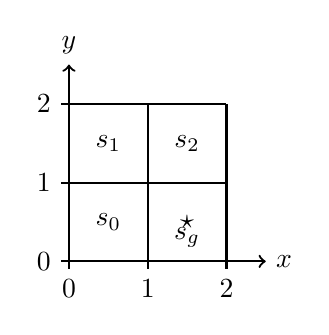
\begin{tikzpicture}
    \tikzstyle{grid}=[draw, thick, fill=gray!10]
    
    % Draw grid
    \draw[grid] (0,0) grid (2,2);
    
    % Add axes
    \draw[thick, ->] (0,0) -- (2.5,0) node[right] {$x$};
    \draw[thick, ->] (0,0) -- (0,2.5) node[above] {$y$};
    
    % Add tick marks and labels
    \foreach \x in {0,1,2} {
        \draw[thick] (\x,0) -- (\x,-0.1) node[below] {$\x$};
    }
    \foreach \y in {0,1,2} {
        \draw[thick] (0,\y) -- (-0.1,\y) node[left] {$\y$};
    }
    
    % Add state labels clockwise from bottom left
    \node at (0.5,0.5) {$s_0$};
    \node at (1.5,0.5) {$\star$};
    \node at (1.5,0.3) {$s_g$};
    \node at (1.5,1.5) {$s_2$};
    \node at (0.5,1.5) {$s_1$};
\end{tikzpicture}
\caption{A grid world MDP state space: it is a $2\times2$ grid.}
\end{figure}

\begin{figure}[h]
\centering
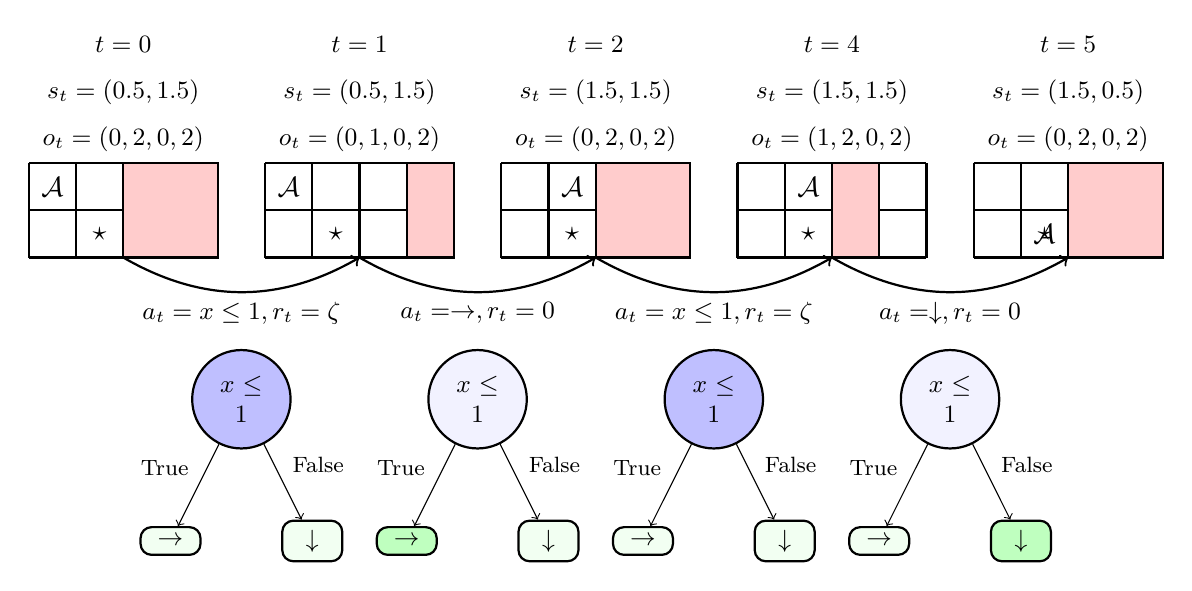
\begin{tikzpicture}[scale=0.6]
    % Define styles
    \tikzstyle{grid}=[draw, thick, fill=gray!10]
    \tikzstyle{rectangle}=[draw, thick, fill=red!20]
    
    % Row 1: IBMDP States (s, o)
    % t=0: Initial state
    \node at (2,8.5) {\small $t=0$};
    \node at (2,7.5) {\small $s_t=(0.5, 1.5)$};
    \node at (2,6.5) {\small $o_t=(0, 2, 0, 2)$};

    \draw[grid] (0,4) grid (2,6);
    \node at (0.5, 5.5) {$\mathcal{A}$};
    \node at (1.5, 4.5) {$\star$};

    \draw[rectangle] (2,4) rectangle (4,6);  
    
    % Curved arrow from t=0 to t=1
    \draw[thick, ->] (2,4) to[bend right=30] node[midway, below] {\small $a_t = x \leq 1, r_t = \zeta$} (7,4);

    % % t=1: After AIG x≤0.5
    \node at (7,8.5) {\small $t=1$};
    \node at (7,7.5) {\small $s_t=(0.5, 1.5)$};
    \node at (7,6.5) {\small $o_t=(0, 1, 0, 2)$};

    \draw[grid] (5,4) grid (7,6);
    \node at (5.5, 5.5) {$\mathcal{A}$};
    \node at (6.5, 4.5) {$\star$};

    \draw[grid] (7,4) grid (9,6);
    \draw[rectangle] (8,4) rectangle (9,6);

    % Curved arrow from t=1 to t=2
    \draw[thick, ->] (7,4) to[bend right=30] node[midway, below] {\small $a_t = \rightarrow, r_t = 0$}(12,4);

    \node[circle, draw, thick, fill=blue!25, text width=2em, text centered, minimum height=1.5em, font=\small] (tree4_root) at (4.5,1) {$x \leq 1$};
    \node[rectangle, draw, thick, fill=green!5, text width=1.5em, text centered, rounded corners, minimum height=1em, font=\small] (tree4_right) at (3,-2) {$\rightarrow$};
    \node[rectangle, draw, thick, fill=green!5, text width=1.5em, text centered, rounded corners, minimum height=1em, font=\small] (tree4_left) at (6,-2) {$\downarrow$};
    \draw[->] (tree4_root) -- (tree4_right) node[font=\footnotesize, midway, above left] {True};
    \draw[->] (tree4_root) -- (tree4_left) node[font=\footnotesize, midway, above right] {False};

    \node at (12,8.5) {\small $t=2$};
    \node at (12,7.5) {\small $s_t=(1.5, 1.5)$};
    \node at (12,6.5) {\small $o_t=(0, 2, 0, 2)$};
    
    \draw[grid] (10,4) grid (12,6);
    \node at (11.5, 5.5) {$\mathcal{A}$};
    \node at (11.5, 4.5) {$\star$};
    \draw[rectangle] (12,4) rectangle (14,6);
    
    % Curved arrow from t=2 to t=4
    \draw[thick, ->] (12,4) to[bend right=30] node[midway, below] {\small $a_t = x \leq 1, r_t = \zeta$} (17,4);

    \node[circle, draw, thick, fill=blue!5, text width=2em, text centered, minimum height=1.5em, font=\small] (tree4_root) at (9.5,1) {$x \leq 1$};
    \node[rectangle, draw, thick, fill=green!25, text width=1.5em, text centered, rounded corners, minimum height=1em, font=\small] (tree4_right) at (8,-2) {$\rightarrow$};
    \node[rectangle, draw, thick, fill=green!5, text width=1.5em, text centered, rounded corners, minimum height=1em, font=\small] (tree4_left) at (11,-2) {$\downarrow$};
    \draw[->] (tree4_root) -- (tree4_right) node[font=\footnotesize, midway, above left] {True};
    \draw[->] (tree4_root) -- (tree4_left) node[font=\footnotesize, midway, above right] {False};

    
    \node at (17,8.5) {\small $t=4$};
    \node at (17,7.5) {\small $s_t=(1.5, 1.5)$};
    \node at (17,6.5) {\small $o_t=(1, 2, 0, 2)$};

    \draw[grid] (15,4) grid (17,6);
    \node at (16.5, 5.5) {$\mathcal{A}$};
    \node at (16.5, 4.5) {$\star$};
    \draw[grid] (17,4) grid (19,6);
    \draw[rectangle] (17,4) rectangle (18,6);
    
    \draw[thick, ->] (17,4) to[bend right=30] node[midway, below] {\small $a_t = \downarrow, r_t = 0$} (22,4);
    
    \node[circle, draw, thick, fill=blue!25, text width=2em, text centered, minimum height=1.5em, font=\small] (tree4_root) at (14.5,1) {$x \leq 1$};
    \node[rectangle, draw, thick, fill=green!5, text width=1.5em, text centered, rounded corners, minimum height=1em, font=\small] (tree4_right) at (13,-2) {$\rightarrow$};
    \node[rectangle, draw, thick, fill=green!5, text width=1.5em, text centered, rounded corners, minimum height=1em, font=\small] (tree4_left) at (16,-2) {$\downarrow$};
    \draw[->] (tree4_root) -- (tree4_right) node[font=\footnotesize, midway, above left] {True};
    \draw[->] (tree4_root) -- (tree4_left) node[font=\footnotesize, midway, above right] {False};


    \node at (22,8.5) {\small $t=5$};
    \node at (22,7.5) {\small $s_t=(1.5, 0.5)$};
    \node at (22,6.5) {\small $o_t=(0, 2, 0, 2)$};
 
    \draw[grid] (20,4) grid (22,6);
    \node at (21.5, 4.5) {$\mathcal{A}$};
    \node at (21.5, 4.5) {$\star$};
    \draw[rectangle] (22,4) rectangle (24,6);

    \node[circle, draw, thick, fill=blue!5, text width=2em, text centered, minimum height=1.5em, font=\small] (tree4_root) at (19.5,1) {$x \leq 1$};
    \node[rectangle, draw, thick, fill=green!5, text width=1.5em, text centered, rounded corners, minimum height=1em, font=\small] (tree4_right) at (18,-2) {$\rightarrow$};
    \node[rectangle, draw, thick, fill=green!25, text width=1.5em, text centered, rounded corners, minimum height=1em, font=\small] (tree4_left) at (21,-2) {$\downarrow$};
    \draw[->] (tree4_root) -- (tree4_right) node[font=\footnotesize, midway, above left] {True};
    \draw[->] (tree4_root) -- (tree4_left) node[font=\footnotesize, midway, above right] {False};

    

    
\end{tikzpicture}
\caption{An IBMDP trajectory when the base MDP is 2$\times$2 grid world, and equivalent decision tree policy traversal. At $t=0$, the agent is in $s_1 = (0.5, 1.5)$. The initial observation is always the base MDP state bounds, here $(0, 2, 0, 2)$ because the base states are in $[0, 2] \times [0, 2]$. The agent takes an information gathering action in $A_{info}$ that tests the feature $x$ of the states against the value $1$. For that, the agent receives reward $\zeta$. This transition corresponds to going through an internal node in a decision tree policy as illustrated in the figure. At $t=1$, after gathering the information that the $x$-value of the current base state is below 1, the observation is updated with the refined state bounds $o_t=(0, 1, 0, 2)$ and the base state remains unchanged. The agent then takes a base action that is to move right. This gives a reward 0, reinitialized the observation to the original bounds, and changes the base state to $s_t=(1.5, 1.5)$. And the trajectory continues like this until the agent reaches the absorbing state $s_g=(1.5, 0.5)$.}
\label{fig:poibmdp_trajectory}
\end{figure}



\subsection{Partially Observable IBMDPs}

Now we know that to find a decision tree policy for a given MPD $\mathcal{M}$ satisfying the definition (cite); one has to find a partially observable--sometimes called \textit{memoryless} or \textit{reactive}--deterministic policy for an IBMDP $\mathcal{M}_{IB}$.
Such problems are classical instances of Partially Observable Markov Decision Processes (POMDPs) (cite). This connection with POMDP was not done by the authors of IBMDPs. 

\begin{definition}[Partially Observable Markov Decision Processes]
A Partially Observable Markov Decision Process (POMDP) is a tuple $\langle X, A, O, T, T_0, \Omega, R\rangle$ where:
\begin{itemize}
    \item $X$ is the state space (like in the base definition of MDPs).
    \item $A$ is a finite set of actions (like in the base definition of MDPs).
    \item $O$ is a set of observations.
    \item $T: X \times A \rightarrow \Delta X$ is the transition kernal, where $T(s, a, x') = P(x'|x, a)$ is the probability of transitioning to state $x'$ when taking action $a$ in state $x$
    \item $T_0$: is the intial distribution over states. 
    \item $\Omega: X \rightarrow \Delta O$ is the observation kernel, where $\Omega(x', a, o) = P(o|x', a)$ is the probability of observing $o$ in state $x$
    \item $R: X \times A \rightarrow \mathbb{R}$ is the reward function, where $R(x, a)$ is the immediate reward for taking action $a$ in state $x$
\end{itemize}
Note that $\langle X, A, R, T, T_0 \rangle$ defines an MDP (cite).
\end{definition}

We can simply extend the definition of Iterative Bounding MDPs (cite) with an observation kernel to get Partially Observable IBMDPs:
\begin{definition}[Partially Observable Iterative Bounding Markov Decision Processes] a Partially Observable Iterative Bounding Markov Decision Process (POIBMDP) is a an IBMDP (cite) extended with an observation kernel 
    \begin{align*}
        \langle \overbrace{S, \underbrace{O}_{\text{Observations}}}^{\text{fully observable states X}}, \underbrace{A, A_{info}}_{A}, \overbrace{R, \zeta}^{R}, \underbrace{T_{info}, T, T_0}_{T, T_0}, \Omega \rangle
    \end{align*}
\end{definition}

The sole specifity of POIBMDPs compared to the general definition of POMDPs, is that $\Omega(o|(s, o'))$, the probability of observing $o$ in $(s,o')$, is $1_{o=o'}$.
This particular instance of POMDPs with observations being some indices of the fully-observable states has other names in the litterature: Mixed Observability MDPs (cite), Block MDPs (cite).
POIBMDPs can also be seen as non-stationary MDPs in which there is one different transition kernel per base MDP state: these are called Hidden-Mode MDPs (cite). 

Following (cite) we can write the definition of the value of a deterministic partially observable policy $\pi:O\rightarrow A$ in observation $o$.

\begin{definition}[Partial observable value function] In a POIBMDP, the expected cumulative discounted reward of a deterministic partially observable policy $\pi:O\rightarrow A\cup A_{info}$ starting from observation $o$ is $V^{\pi}(o)$:
    \begin{align*}
        V^{\pi}(o) &= \underset{(s,o')\in S\times O}{\sum}P^{\pi}((s, o')|o)V^{\pi}((s, o'))
    \end{align*}
with $P^{\pi}((s, o')|o)$ the asymptotic occupancy distribution (see cite for definition) of the fully observable state $(s,o')$ given the partial observation $o$ and $V^{\pi}((s, o'))$ the classical state-value function defined in (cite).
\end{definition}


The asymptotic occupancy distribution is the probability of a policy $\pi$ to be in $(s,o')$ while observing $o$ and having taken actions given by $\pi$.  

The problem that we solve is to find the deterministic partially observable policy that maximizes the excpeted value in the initial observation:
\begin{align}
    \pi^{\star} &= \underset{\pi}{\operatorname{argmax}}J(\pi) = \underset{\pi}{\operatorname{argmax}}V^{\pi}(o_0)
\end{align}
With $\pi:O\rightarrow A\cup A_{info}$. There is no expectation over possible initial observation in the above objective function as there is only one initial observation in a POIBMDP: $o_0=(L_1, U_1, \dots, L_n, U_n)$.

This particular problem of learning deterministic partially observable policies for POMDPs has been studied in the works of Littman, Singh and Jordan: (cite).
In (cite) atuhors give som intution behind why the above optimization problem is hard. For example, the optimal partially observable policy can be stochastic (cite precise section), hence policy gradient algoriothms (cite) are to avoid. 
Furthermore, the optimal deterministic patially observable policy might not maximize all the value of all observations simulataneously (cite precise section) which makes difficult the use the Bellman optimality equation (cite) to compute policies.
Despite those hardness results, empirical results of applying RL to POMDPs by naively setting the states to be observations has shown promising results (cite). 
More recently, the framework of Baisero et. al. (cite) called asymmetric RL has also shown promising empirical and theoretical results when leveraging fully-observable state information during training of a partially observable policy.
In the next chapter, we use reinforcement learning to train decision tree policies for MDPs by seeking deterministic partially observable policies for POIBMDPs (cite).  
\begin{figure}[h]
\centering
\begin{tikzpicture}
    \draw[fill=blue!40] (0, 0) rectangle (6, 4);
    \node at (3, 3.5) {POIBMDP $\mathcal{M}_{POIB}\langle\mathcal{M}_{IB}, \Omega\rangle$};
    \draw[fill=blue!30] (0, 0) rectangle (5.9, 3);
    \node at (3, 2.5) {IBMDP $\mathcal{M}_{IB} \langle \mathcal{M}, O, A_{info}, \zeta, T_{info}\rangle$};
    \draw[fill=blue!10] (0, 0) rectangle (5, 2);
    \node at (3, 1.5) {MDP $\mathcal{M} \langle S, A, R, T, T_0 \rangle$};
    
    \draw[fill=red!10] (10, 0) rectangle (14, 3);
    \node at (12, 2) {\textbf{Objective}};
    \node at (12, 1) {$\pi^{\star} = \underset{\pi}{\operatorname{argmax}} V^{\pi}(o_0)$};
    
    \draw[fill=red!10] (1, -5) rectangle (5, -2);
    \node at (3, -3) {\textbf{Decision Tree Policy}};
    \node at (3, -4) {$\pi_{\mathcal{T}}: S \rightarrow A$};
    
    \draw[fill=red!10] (9.5, -5) rectangle (14.5, -2);
    \node at (12, -3) {\textbf{Deterministic PO Policy}};
    \node at (12, -4) {$\pi: O \rightarrow A \cup A_{info}$};
    
    \draw[thick, ->] (6, 2) -- (10, 2) node[midway, above] {$\gamma$};
    \draw[thick, <-] (5, -3.5) -- (9.5, -3.5) node[midway, above] {Extract tree with Alg 6};
    \draw[thick, ->] (12, 0) -- (12, -2) node[midway, left] {Solve with e.g. RL};
    \draw[thick, <-] (3, 0.5) -- (3, -2) node[midway, left] {Can be interpreted};

    
    % % Final arrow from tree back to base MDP - adjusted position
    % \draw[thick, ->] (1.75, -2.5) -- (1.75, -0.5) node[midway, right] {Can deploy\\and interpret};
    
\end{tikzpicture}
\caption{A formal framework to learn decision tree policies for MDPs. This include learning a partially observable deterministic policy in a POIBMDP (cite).}
\label{fig:nested_decision_processes}
\end{figure}

